\documentclass{article}
\title{\textbf{Trabajo Práctico Nº1 - Inter Process Communication} \\ [1ex]
\large Instituto Tecnológico de Buenos Aires - Sistemas Operativos (72.11) \\ [1ex]
\large Grupo  }
\date{14 de septiembre de 2024}
\author{
\textbf{Ignacio Searles}\\
isearles@itba.edu.ar\\
64.536
\and
\textbf{Augusto Barthelemy Solá}\\
abarthelemysola@itba.edu.ar\\
64.502
\and
\textbf{Santiago Bassi}\\
sabassi@itba.edu.ar\\
64.643
}

\usepackage{multicol}
\usepackage{graphicx, wrapfig}
\graphicspath{ {imagenes/} }

\usepackage{float}
\usepackage{amsmath}
\usepackage{amsfonts}

\usepackage{caption, threeparttable}
\usepackage{hyperref}

\usepackage[margin=1.3in]{geometry}

\usepackage{listings}

\renewcommand{\figurename}{Figura}
\renewcommand{\tablename}{Tabla}
\renewcommand*\abstractname{Resumen}

\begin{document}
\maketitle

\begin{abstract}
El siguiente informe expone los apectos fundamentales del Trabajo Práctico Nº1 - Inter Process Communication (IPC). El trabajo consiste en la distribución y manejo de trabajos, por un proceso master, a diferentes procesos slaves; como así también, la subsiguiente visualización de las salidas de los trabajos mediante un proceso de vista.
\end{abstract}

\section{Decisiones de diseño}

\subsection{Master}
Se optó por construir la aplicación en funciones pequeñas, lo que permite una mayor versatilidad y modularidad en el diseño. Inicialmente, a cada esclavo se le asigna una cantidad de archivos configurada mediante la macro NUM\_FILES\_IN\_INITIAL\_JOB. A medida que los esclavos completan su trabajo, se les asignan nuevos archivos uno por uno hasta que todos han sido procesados. Este enfoque se eligió para evitar situaciones en las que un esclavo recibe archivos pesados y otro archivos livianos, lo que podría causar que uno termine rápidamente mientras el otro continúa trabajando, desperdiciando así capacidad de procesamiento.

Además, los resultados generados por los esclavos se almacenan tanto en un archivo de salida como en un buffer compartido mediante el uso de memoria compartida. Esto permite que, si el proceso view se ejecuta, pueda acceder a la información necesaria para mostrar los datos en tiempo real.

Finalmente, el código incorpora un manejo básico de errores en cada etapa crítica, como la creación de pipes, la duplicación de descriptores de archivos y la creación de procesos. Esto garantiza que el sistema pueda reaccionar adecuadamente ante posibles fallos, minimizando su impacto y facilitando la depuración.

\subsection{Slaves}
Los procesos esclavos son los encargados de calcular el hash MD5 de los archivos. Para ello, emplean el programa md5sum, que toma como parámetro el nombre de un archivo y genera su hash correspondiente. Hemos optado por que los esclavos lean los nombres de los archivos a procesar desde la entrada estándar y, posteriormente, impriman el hash resultante en la salida estándar. Este enfoque permite que, una vez que el esclavo está en ejecución, podamos enviarle nuevos archivos a medida que finaliza con los anteriores, lo cual no sería posible si los archivos se proporcionaran como parámetros al iniciar el proceso.

\subsection{View}

El proceso view se encarga de leer los datos que el proceso aplicación escribe en el buffer de memoria compartida y mostrarlos en pantalla. En el buffer de memoria compartida guardamos estructuras con la información de salida de cada archivo procesado. Al utilizar memoria compartida, es esencial abordar el problema de las condiciones de carrera, que pueden surgir cuando múltiples procesos acceden concurrentemente a los mismos recursos. Para mitigar este riesgo, se implementaron semáforos como mecanismo de sincronización. Además, se decidió leer los nombres del semáforo y del búfer desde la entrada estándar, lo que confiere mayor flexibilidad al proceso view, permitiendo su reutilización en futuros escenarios con cambios mínimos.

\subsection{Comunicación entre procesos}

El proceso master se comunica con los procesos slaves mediante pipes. Por cada slave existen dos pipes, un pipe de entrada al slave y otro pipe de salida del slave. El master utiliza select(2) para determinar si alguno de los pipes de salidas tiene datos para ser leídos, podiendo así determinar cuando el slave termina de procesar un archivo del trabajo. Luego, el proceso master se comunica con el proceso view mediante un shared buffer, para evitar condiciones de carrera se emplean semáforos. (Ver figura \ref{fig:diagramaComunicacion})

\begin{figure}[H]
\begin{center}
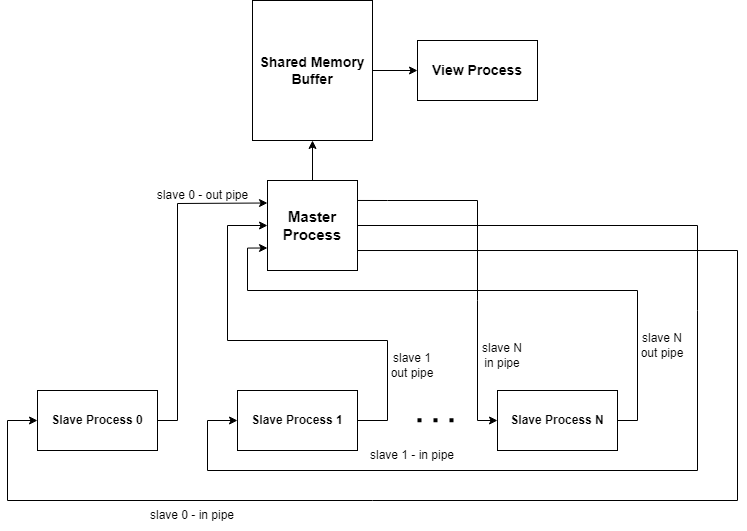
\includegraphics[width=70mm]{diagramaComunicacion}
\caption{Diagrama donde se observa la comunicación entre procesos.}
\label{fig:diagramaComunicacion}
\end{center}
\end{figure}

\section{Compilación y ejecución}

El trabajo práctico fue compilado y ejecutado utilizando la imagen de docker provista por la cátedra. Dentro del contenedor puede ejecutarse los siguientes comandos para compilar el proyecto.

\begin{lstlisting}[language=bash]
$> make clean
$> make
\end{lstlisting}
Una vez compilado, puede ejecutarse el programa principal mediante el siguiente comando.

\begin{lstlisting}[language=bash]
$> ./app file1 file2 ... fileN
\end{lstlisting}
Para también correr el proceso de vista, junto con el programa principal, usando un pipe se puede ejecutar el siguiente comando.
\begin{lstlisting}[language=bash]
$> ./app file1 file2 ... fileN | ./view
\end{lstlisting}
El proceso vista puede ser ejecutado de forma independiente del proceso principal, si el proceso principal está corriendo, se puede ejecutar el proceso vista y ingresar el nombre del semaforo  por teclado (provisto por salida estandar cuando se ejecuta ./app).
\begin{lstlisting}[language=bash]
$> ./view
/md5view
\end{lstlisting}
Siendo /md5view el nombre asignado al semaforo y al objeto de memoria compartida (modificable en app.h).

\section{Limitaciones}

Una de las principales limitaciones del sistema es la eficiencia en la asignación de trabajos. Actualmente, el sistema asigna archivos a los esclavos de uno en uno después de una carga inicial, lo cual puede no ser óptimo cuando los archivos tienen tamaños similares. Para mejorar el rendimiento y la utilización de los recursos, especialmente en entornos con archivos de tamaños uniformes, sería beneficioso implementar un mecanismo más dinámico para la asignación de trabajos.

Otra limitación relevante es la flexibilidad en el manejo de errores. Aunque el sistema incluye un manejo básico de errores, fortalecer la capacidad para detectar y gestionar fallos en la comunicación entre el proceso principal y los esclavos podría aumentar la robustez del sistema. Incorporar mecanismos de reintento o procedimientos de recuperación ayudaría a minimizar el impacto de errores y a mejorar la estabilidad general del sistema.

Además, el diseño actual del sistema está limitado a recibir únicamente una lista de archivos. Una mejora significativa sería permitir que el sistema acepte directorios completos, procesando todos los archivos contenidos en cada uno de los subdirectorios. Esta expansión en la funcionalidad permitiría una mayor flexibilidad y eficiencia en el manejo de grandes conjuntos de datos organizados en estructuras de directorios.

\section{Problemas enfrentados}

Uno de los problemas enfrentas fue el de manejar la sincronización en app con los esclavos. Como planteamos un diseño donde cada trabajo puede tener más de una tarea (en este caso procesar un archivo), tuvimos inicialmente el problema de que los esclavos procesaban una cantidad variable de tareas cada vez que checkeabamos el pipe desde main. Por este motivo planteamos un seguimiento del trabajo actual para cada esclavo. Teniendo en cuenta la cantidad de tareas a realizar y la cantidad de tareas realizadas.

Otro problema enfrentado fue determinar desde view cuando app terminaba de procesar. El problema es que sem\_wait es una llamada bloqueante, por más que cerremos el semáforo sem\_wait quedaba bloqueado. Para solucionar este problema, introducimos una estructura nula que indica que app terminó. 

\end{document}
